\justify
\textcopyright{} 2021, by Franklin Diaz
\justify
All rights reserved. This book or any portion thereof
may not be reproduced or used in any manner whatsoever
without the express written permission of the publisher
except for the use of brief quotations in a book review.
\vspace{5mm}\\
First Edition 2021
\justify
Front cover image of the Plouzane Lighthouse France and images
at the beginning of the chapters in this book are
\href{https://pixabay.com/service/terms/#license}{courtesy of Pixabay}
\justify
Follow along code project available from {\href{https://github.com/hotpeppersec/rapid_secdev_framework}{RapidSecDevFramework}}
\vspace{3mm}
Published on: \today

\justify
This book was drafted using the reStructuredText file format. 
The Sphinx module for Python was used to format these files and programatically
generate LaTeX, and other working formats used in the typesetting process. The
resultant LaTeX files were manged using TeXstudio.

Some graphs have been generated programatically using the Graphviz software. 
The entire publishing environment is encapsulated in a container according
to the principles outlined in this book.

\vspace{5mm}
    \centering
\vspace{0mm}
\begin{figure}[!htb]
	\centering
	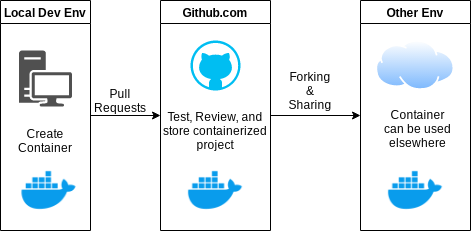
\includegraphics[scale=0.75]{../images/workflow.png}
\end{figure}
\vspace{2mm}
Containerized publishing workflow.
